\section{\nb{Interpretation: a Theory Model of the Boundary and the Optimum Step}}
\label{sec:theory}
\begin{newtext}
\Cref{sec:p3,sec:muopt} report measurements. This section derives them from first-order LMS theory applied to the actual channel, with no fitted constant and no LMS simulation, so that every headline number has two independent sources.

\subsection{Model}
Following the two terms of \eqref{eq:mis}, R3's excess MSE is split into lag and gradient noise, each computed for the real trajectory instead of a random walk.
\emph{Lag.} Under the usual independence assumption the mean coefficient vector obeys the deterministic recursion
\begin{equation}
\bar{\mathbf w}[n+1]=\bar{\mathbf w}[n]+\mu\big(\mathbf p[n]-\mathbf R[n]\,\bar{\mathbf w}[n]\big),
\label{eq:meanw}
\end{equation}
started from the Wiener filter of the training channel, where $\mathbf R[n]$ and $\mathbf p[n]$ are the exact moving-window statistics of the time-varying channel (the same as the oracle's). The lag excess $\varepsilon_{\rm lag}(\mu,S)$ is $J_n(\bar{\mathbf w}[n])-J_{\rm or}[n]$, averaged over the evaluation window and divided by the mean oracle MSE.
\emph{Gradient noise.} The correlated-error result \eqref{eq:corrmis}, computed for every channel state and averaged over the time the triangle spends there: $\varepsilon_{\rm gn}(\mu)\propto\mu$.
\emph{Predictions.} $\varepsilon=\varepsilon_{\rm lag}+\varepsilon_{\rm gn}$; $\rho=\varepsilon_{\rm lag}/(\varepsilon_{\rm plateau}-\varepsilon_{\rm gn})$; $S^\star_{\rm MSE}$ as the fastest grid rate with $\rho<0.5$ (the measurement rule, without the bootstrap), and the continuous crossing $x^\star$ where $\rho=0.5$ exactly; $\mu_{\rm opt}(S)=\arg\min_\mu\varepsilon$. A \emph{semi-empirical} variant uses the measured static excess in place of $\varepsilon_{\rm gn}$, to test the lag part alone.

\subsection{Agreement with the measurements}
\emph{Boundary:} for $\mu\le2^{-7.5}$ the pure-theory model gives the measured $S^\star_{\rm MSE}$, at the resolution of the rate grid, \textbf{in all 40 cases} (2 channels $\times$ 14 and 16\,dB $\times$ 10 step sizes; \cref{fig:model}a). For $\mu\ge2^{-7}$ it is mostly one grid step too fast, and at $\mu=2^{-5}$ up to three steps, because the first-order gradient noise is too small there (by a factor 0.48--0.65); the semi-empirical variant removes most of that error. \emph{Lag:} predicted/measured lag excess has median 0.98 (10--90\,\%: 0.84--1.00) over 143--177 points per case. \emph{Exponent} (\cref{fig:muopt}b): the semi-empirical model gives 0.512, 0.505, 0.591 and 0.575 against the measured 0.519, 0.525, 0.593 and 0.575 (primary 16/14\,dB, control 16/14\,dB), within 0.02 and with the right channel dependence; pure theory gives 0.573, 0.570, 0.623 and 0.607, 0.03--0.05 too high for the same large-$\mu$ reason --- the finite-step effect also found in replication R6.

\begin{figure*}[t]
\centering
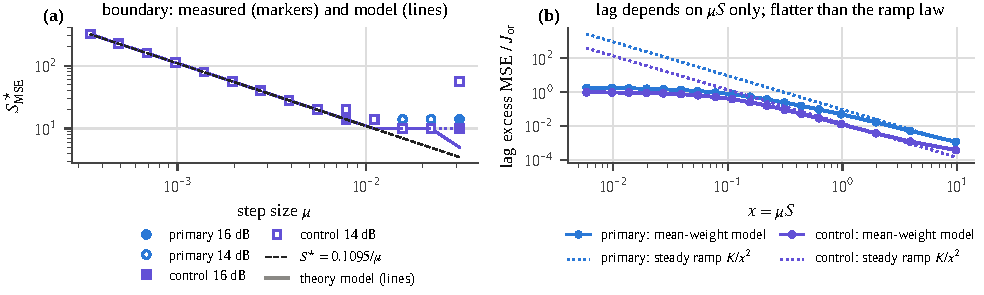
\includegraphics[width=\linewidth]{figs/model.pdf}
\caption{Theory model against measurement (\lvl{L1}; the model runs no LMS simulation). (a)~$S^\star_{\rm MSE}$ against $\mu$, measured (markers) and pure-theory model (lines), with $S^\star=0.1095/\mu$; for $\mu\le2^{-7.5}$ the model gives the measured grid point in all 40 cases. (b)~Lag excess against $x=\mu S$ from the mean-weight model at $\mu=2^{-9}$, with the steady-ramp law $K/x^2$ (dotted): the lag depends on $\mu S$ only, and on the primary channel it falls much more slowly than the ramp law, which is why the exponent is below 2/3.}
\label{fig:model}
\end{figure*}

\subsection{Why $S^\star_{\rm MSE}\propto1/\mu$}
In \eqref{eq:meanw} the channel moves one counter step every $S$ symbols while the filter moves at rate $\mu$. Rescaling time by $S$ shows that the lag depends on $\mu$ and $S$ almost only through
\begin{equation}
x=\mu S,
\label{eq:x}
\end{equation}
the adaptation progress made per channel step (checked: $\varepsilon_{\rm lag}$ at fixed $x$ changes by at most 2\,\% between $\mu=2^{-8}$ and $2^{-10}$). When the gradient noise is small compared with the plateau, $\rho\approx\varepsilon_{\rm lag}(x)/\varepsilon_{\rm plateau}$, so the boundary is a fixed $x^\star$:
\begin{equation}
S^\star_{\rm MSE}\approx x^\star/\mu,\qquad x^\star\approx0.082\text{--}0.087,
\label{eq:law}
\end{equation}
for both channels and both SNRs (on the measurement grid the last passing point gives $S^\star\mu=0.109$--0.110; the two constants describe the same boundary, because the last passing grid point lies up to one grid step, a factor of about 1.4, on the slow side of the continuous crossing). In words: \emph{the equalizer keeps up as long as it makes enough adaptation progress per channel step, and accuracy is lost when $\mu S$ falls below about 0.085.} This is why the boundary is set by $\mu$ and not by the SNR or the channel. For large $\mu$ the gradient noise uses up part of the room below the plateau, so the boundary moves to slower variation, and $\rho$ becomes undefined at $\mu=2^{-5}$, 12--14\,dB.

\subsection{Why the exponent is about 0.52}
Near the optimum write $\varepsilon\approx G(\mu S)+\kappa\mu$ with $G\propto(\mu S)^{-q}$ locally. Setting ${\rm d}\varepsilon/{\rm d}\mu=0$ gives
\begin{equation}
\mu_{\rm opt}\propto S^{-q/(q+1)}.
\label{eq:qrule}
\end{equation}
A steady ramp has $q=2$ (exponent 2/3); a random walk has $q=1$ (exponent 1/2). The measured exponent therefore tells how steeply the lag falls with $\mu S$ at the optimum. In the model, $q$ falls from about 1.7 at slow variation to about 0.9--1.1 at fast variation on the primary channel ($q/(q+1)$ from 0.63 to 0.48), and from 1.8 to 1.2--1.4 on the control channel (0.64 to 0.54--0.59); the fitted exponent is the average, and the falling $q$ is the curvature seen in the measurements.

\emph{Why $q<2$.} The steady-ramp law assumes that every eigen-direction of $\mathbf R$ has settled; direction $i$ settles with time constant $1/(\mu\lambda_i)$. On the primary channel $\lambda_{\min}$ falls from 0.63 ($c=40$) to \textbf{0.071} ($c=116$), an eigenvalue spread of up to 56. At the measured optimum this slowest direction completes only about 0.8--18 time constants per half period of the triangle (17.6 at $S=5000$, 1.7 at $S=28$, 0.8 at $S=10$) before the ramp turns round. The lag is therefore smaller than the steady-ramp value (0.12 of it at $x\approx0.1$) and falls more slowly with $\mu S$, so $q<2$ (\cref{fig:model}b). The control channel is better conditioned ($\lambda_{\min}\ge0.27$, spread $\le11$; 2.3--30 time constants), so $q$ stays nearer 2 and its exponent is larger.

\emph{Consequence for \eqref{eq:mis}.} Its structure --- an interior optimum that grows with the variation rate --- is confirmed. Its exponent is not universal --- Widrow \etal already note that the lag is ``quite sensitive to the spectral characteristics of the fluctuation \cite[footnote~4]{widrow1976} ---: it depends on the channel's eigenvalue spread and on how far the trajectory is from a steady ramp. On the primary channel the measured exponent is consistent with the ``square root'' within its systematic uncertainty, but this is a coincidence of $q\approx1$ near the optimum, not evidence of random-walk behaviour; the control-channel value shows that the exponent changes with the channel, and two channels are not enough to state a general rule.

\subsection{What kind of statement each result is}
\Cref{tab:claims} separates exact results, first-order approximations, fitted trends and agreement at grid resolution, so that each number is read with the right strength.

\begin{table}[t]
\centering\small
\caption{\nb{Status of the main quantitative claims.}}
\label{tab:claims}
\color{blue}
\setlength{\tabcolsep}{3pt}
\begin{tabular}{@{}p{0.47\linewidth}p{0.47\linewidth}@{}}
\toprule
Claim & Type\\
\midrule
Misadjustment ratio 1.468, \eqref{eq:corrmis} & first order in $\mu$; $C(j)$ computed exactly from the channel\\
Lag depends on $x=\mu S$ only & approximation (mean-weight model); checked to 2\,\%\\
$x^\star\approx0.082$--0.087 & model prediction of the continuous crossing $\rho=0.5$\\
$S^\star_{\rm MSE}\mu=0.109$--0.110 & measured; last passing grid point\\
Model = measurement in 40 cases & agreement at the resolution of the rate grid\\
$\mu_{\rm opt}\propto S^{-q/(q+1)}$ & local power-law approximation near the optimum\\
Exponents 0.52 and 0.58--0.59 & fitted trends; systematic band about $\pm0.03$\\
$q<2$ from the slowest eigen-direction & explanation supported by the model, for these two channels\\
\bottomrule
\end{tabular}
\end{table}

\subsection{Limits of the model}
The model is first-order (independence) theory, and its gradient-noise term is too small at large $\mu$; the best exponent agreement uses the measured static excess. At the smallest $\mu$ the measured static excess also exceeds the first-order value (theory/measured 0.26--0.84); this is not yet explained. BER boundaries are not modelled, and the model is \lvl{L1}; a fixed-point version would add the stall term of \cref{sec:fxp}.
\end{newtext}
